\thispagestyle{empty}
\chapter{Assessing Ruby on Rails Projects}\label{chap:assissing_ror}

To assess the quality of a software project is not an easy task.
Too many variables should be taken into consideration and most of their values can be considered subjective.

Our thesis is that the quality of an open source project is somehow influenced by the best practices followed 
by its contributors.

Furthermore, since the Rails community has been our object of study, we have decided to conduct a series of studies 
with the objective of finding correlations between best practices defined by the Rails community and
the quality of projects following it.

With the objective of being able to automatically verify whether or not best practices are being followed by
a given Rails project, the open source ruby gem rails\_best\_practices 
was created (by the authors of Rails best practices web site).
We agreed on using it as the starting point for our work.

This chapter reports the different studies carried out, the main difficulties, and the results obtained.



\section{First Study}\label{subsec:first_study}
One of the first things that we have noticed, when we applied the rails\_best\_practices gem to OSS projects,
is that the biggest and most renowned projects have much more errors than the smaller and unknown projects.
This apparent nonsense has a simple  interpretation.
Small projects (like the majority of Rails projects found in GitHub) are simple software packages,
often developed by a single user, and are carried out for simple learning purposes.
These applications are so simple that many times the code is almost entirely created by Rails code generators.
Usually, when code is not written by humans, it has few mistakes concerning those recommendations.

Having taken the above into account, we decided to run the rails best practices gem on similar Rails projects.
Seven \emph{time tracking} or \emph{project management} open source systems were chosen.
After running the gem and counting the
\textsf{not best practices (NBPs)}\footnote{In fact, Rails Best Practices gem does not find best practices in the source code.
  It does the opposite, it discovers when the code is not written according to a best practice, in other words, 
  it identifies bad practices (similar to the detection of code smells).
  We decided to name those occurrences NBP.
}
occurrences, the following results were obtained:

\begin{table}[H]
\begin{center}{\scriptsize
  \begin{threeparttable}
  \begin{tabular}{|l||c|c|c|c|c|c|c|} \hline
  \multicolumn{8}{|c|}{Rails Best Practices Results} \\ \hline
  \textbf{Best Practice}& \textbf{A}& \textbf{B}& \textbf{C}&  \textbf{D}& \textbf{F}& \textbf{G}& \textbf{H} \\\hline\hline
  \emph{\tnote{a}Add model virtual attribute           }              &   -  &   2  &   7  &   - &   - &   5 &   4  \\ \hline
  \emph{Always add db index                   }              &   -  &   -  &   -  &  43 &   - &   - &  51  \\ \hline
  \emph{Isolate seed data                     }              &   -  &   -  &   -  &   - &   - &  79 &  17  \\ \hline
  \emph{Law of demeter                        }              &  20  &  38  &  45  &   6 &  30 & 164 &  85  \\ \hline
  \emph{Move code into controller             }              &   -  &   -  &   -  &   - &   2 &   - &   4  \\ \hline
  \emph{Move code into model                  }              &   -  &  26  &   -  &   7 &   1 &   3 &  19  \\ \hline
  \emph{Move model logic into model           }              &   -  &   -  &  76  &  11 &  11 &  98 & 100  \\ \hline
  \emph{Move finder to named\_scope           }              &   -  &   4  &   9  &   2 &   4 &  25 &   -  \\ \hline
  \emph{Needless deep nesting                 }              &   -  &   -  &   -  &   1 &   - &   - &   -  \\ \hline
  \emph{Not use default root                  }              &   -  &   1  &   1  &   - &   1 &   1 &   1  \\ \hline
  \emph{Notes  use query attribute            }              &   -  &   2  &   -  &   - &   - &   - &   -  \\ \hline
  \emph{Overuse route customizations          }              &   -  &   -  &   2  &   4 &   - &   2 &   2  \\ \hline
  \emph{Remove trailing whitespace            }              &  68  &  57  & 126  & 110 & 330 & 316 & 100  \\ \hline
  \emph{Use factory method                    }              &   -  &  15  &   9  &   5 &   1 &   8 &  19  \\ \hline
  \emph{Replace instance var with local var   }              &  13  &   -  &  70  & 239 & 142 &  31 & 100  \\ \hline
  \emph{Use before\_filter                    }              &   -  &   7  &   9  &   8 &   8 &  19 &  23  \\ \hline
  \emph{Wrong email content\_type             }              &   -  &   3  &   -  &   - &   - &   - &   -  \\ \hline
  \emph{Use query attribute                   }              &   -  &   -  &  11  &   5 &   8 &  29 &   6  \\ \hline
  \emph{Use say with time in migrations       }              &   -  &   -  &  24  &   - &  10 &  23 &  56  \\ \hline
  \emph{Use scopes access                     }              &   -  &   -  &   -  &   - &   - &   - &  04  \\ \hline
  \emph{User model association                }              &   -  &   -  &  12  &   9 &   - &   1 &  21  \\ \hline
  \emph{Keep finders on their own model       }              &   8  &   4  &   1  &   - &  11 &   - &   -  \\ \hline
  \emph{Total                                 }              & 109  & 156  & 402  & 450 & 559 & 834 & 864  \\ \hline
  \end{tabular}
  \begin{tablenotes}
	\item Results obtained by running the \emph{best practices analyzer gem} on the 7 Open Source Projects chosen 
	      (data produced on April, 2011).
    \item \emph{A:} Rubytime
    , \emph{B:} Notes
    , \emph{C:} Tracks
    , \emph{D:} Handy Ant
    , \emph{F:} Retrospectiva
    , \emph{G:} Redmine
    , \emph{H:} Clockingit
    \item Figures shown represent the number of times a project do not follow a best practice; is expected that \emph{smaller the number, better the project}.
  \end{tablenotes}
  \end{threeparttable}
}
\end{center}
\caption{Best practices analyzer gem raw results using 7 open source projects}
\end{table}

Rubytime seems to have the best results and Clockingit the worst. 
The fact is that very good user reviews can be found about Rubytime.
However, Tracks obtained an unexpected high score, since it has been very sparsely maintained 
(old code has higher probability of not following the current best practices).
As explained before, those values are not really measuring if a project follows best practices ,
but instead measuring when it fails.
This should also be taken into consideration. 

The most evident problem here is that best practices are not being weighted, and the size of the project is not being considered.
For instance, if the developers have the habit of leaving trailing white spaces, this will obviously be related to the size of the project.
On the other hand, it is a best practice to remove the default route generated by rails; 
independent of the project size this is either true or false: there is no way to leave the route two times. 
So, if developers do not take into account the differences between these two best practices, when the project grows, 
the number of trailing spaces will increase and the results will show more NBPs. 
However, the other best practice (remove the default route) will always count as only one NBP.  
This can generate twisted results.

To avoid this, the projects were sized.
The size attribute is based on the quantity of models and controllers in the project.
After that, we divided the values previously obtained  by the project size.
Now a new set of results emerge.

\begin{table}[H]
\begin{center}
{\scriptsize
\begin{threeparttable}
\begin{tabular}{|l||c|c|c|c|c|c|c|} \hline
\multicolumn{8}{|c|}{Rails Best Practices Results} \\ \hline
\textbf{Best Practice}& \textbf{A}& \textbf{B}& \textbf{C}&  \textbf{D}& \textbf{F}& \textbf{G}& \textbf{H} \\\hline\hline
\emph{Total                                           }              & 109  & 156  & 402  & 450 & 559 & 834 & 864  \\ \hline
\emph{Total Without Trailing Whitespace               }              &  41  &  99  & 276  & 340 & 229 & 518 & 764  \\ \hline
\emph{Project Size                                    }              &  12  &  11  &  11  &  29 &  26 &  58 &  31  \\ \hline
\emph{Total / Project Size                            }              &   9  &  14  &  37  &  16 &  23 &  15 &  28  \\ \hline
\emph{Total Without Trailing Whitespace / Project Size}              &   3  &   9  &  25  &  12 &   9 &   9 &  25  \\ \hline
\end{tabular}
\begin{tablenotes}
  \item \emph{A:} Rubytime
  ; \emph{B:} Notes
  ; \emph{C:} Tracks
  ; \emph{D:} Handy Ant
  ; \emph{F:} Retrospectiva
  ; \emph{G:} Redmine
  ; \emph{H:} Clockingit
  \item Results obtained by running the \emph{best practices analyzer gem} on the 7 Open Source Projects chosen, 
        after normalization (data produced on April, 2011).
\end{tablenotes}
\end{threeparttable}
}
\end{center}
\caption{Best practices analyzer gem normalized results using 7 open source projects}
\label{tab:rbpresults_1}
\end{table}

Those results (in Table~\ref{tab:rbpresults_1}) are much more likely to be helpful in terms of understanding whether or not a project is following 
best practices.
The numbers reflect both the community reviews and our own estimates much more.



\section{Second Study}\label{subsec:second_study}
After the first study reported above, we felt that it was time to conduct a larger one.
We felt that we should repeat the experiment over a larger sample. 
As a second target for this new phase, it was decided to find an objective quality rate (a reputation ranking) 
for each project in the sample.
There was the need to define an objective quality metric to compare the metrics results with.
This way it would be possible to prove that there is a statistical relationship between the quality of the project
and the results of our best practices metric based on NBPs.

For the second study, we selected 40 Ruby on Rails projects hosted in GitHub and
decided to consider the number of 
\textsf{followers}\footnote{Number of users that want to receive notifications about the project.} and
\textsf{forks}\footnote{Number of people that forked the project. This means that either they want to contribute to the project or create a derived project}, 
that each project has on GitHub, 
as a \emph{project reputation} metric. 

The objective was then to prove that a negative correlation exists between the NBPs of a project and its followers and forks. 

The previous study has shown us the need to apply different weights to each NBP. 
By dividing the NBPs by the size of project, we achieved better results.
However, not all NBPs depend on the project size.
It turned out to be clear, that each NBP should be weighted in a different way depending
on the nature of the best practice related to it, and characteristics of the project.
Therefore, we altered the rails best practices gem to make it possible to know how many project files were analyzed 
by each rails best practice checker.
What this means is that if an NBP checker is just trying to find occurrences of errors in the models files of the project
we will weigh this result based on the number and size of models.
This is not the perfect solution yet, but it gives much better results than dividing all the best practices by the project size.

In the first study, we analyzed 7 projects. Now we have 40, and obviously this time we had to start automating some things.
The work flow to get the information of a project is described in a few steps:
\begin{itemize}
\item \emph{Retrieve GitHub information}. In this step we get the followers and forks(and more info that might be used in further analyses).
\item \emph{Download the project repository}.
\item \emph{Run rails best practices gems}. At this point, we get the non weighted NBPs and files given by each one of the 29 checkers.
\item \emph{Calculate the Weighted Global NBPs}. The evaluation algorithm consists of dividing the value returned by each NBP checker  by the number of files checked, and then summing it.
\end{itemize}

After collecting the GitHub URLs for the 40 projects, we used a script to apply the described steps to each project
and stored all the information about the projects in a CSV table.

\begin{table}[H]
\begin{center}
{\scriptsize
\begin{threeparttable}
\begin{tabular}{|l||c|c|c|c|c|c|c|c|c|c|c|} \hline
\multicolumn{12}{|c|}{Rails Best Practices Results} \\ \hline
Projects & \textbf{Forks}         & \textbf{Watchers} & 
C1       & C1 F.                  & \textbf{W. C1} & 
C2       & C2 F.                  & \textbf{W.       C1} & 
...      & T. NBPs                & \textbf{W.  T. NBPs} \\\hline\hline
\emph{Rails Admin } & 30 & 2478 &  0 & 141 & \textbf{  0 }&  0 &  37 & \textbf{ 0} & ...&  50 & \textbf{ 739}  \\ \hline
\emph{Rubytime    } & 12 &   82 & 24 & 161 & \textbf{149 }&  0 & 134 & \textbf{ 0} & ...& 146 & \textbf{1334}  \\ \hline
\emph{Redmine     } & 30 & 1781 & 49 & 996 & \textbf{ 49 }&  1 & 362 & \textbf{ 2} & ...& 884 & \textbf{1402}  \\ \hline
\emph{BrowserCMS  } & 30 &  784 & 11 & 234 & \textbf{ 47 }&  0 & 216 & \textbf{ 0} & ...& 268 & \textbf{1510}  \\ \hline
\emph{Tracks      } & 17 &   87 & 46 & 842 & \textbf{ 54 }& 15 & 271 & \textbf{55} & ...& 569 & \textbf{2810}  \\ \hline
\emph{...}&...&...&...&...&...&...&...&...&...&...&...\\ \hline
\end{tabular} 

\begin{tablenotes}
  \item Results obtained by running the \emph{best practices analyzer gem} on the 40 Open Source Projects chosen, 
        from GitHub (data produced on April, 2011). The full table can be found at www.study.gorgeouscode.com
  \item{ \emph{C(x): }} The rails best practices gem has 29 checkers(when this study was carried), 
                        each one tries to find occurrences of a different nbp in the project. 
  \item{\emph{C(x) Files: }} The number of files in the project, where it tried to find nbps 
                             (for instance, some checkers may only be concerned with html files, 
                             some other checker nbps my only occur in model files, etc)
  \item{\emph{W. C(x): }} Weighted C(x) = C(X) / C(x)Files * 1000 
                          (A really small number is added to each variable to avoid divisions by zero).
\end{tablenotes}
\end{threeparttable}
}
\end{center}
\caption{Best practices analyzer gem results using 40 open source projects}
\label{tab:rbpresults_2_raw}
\end{table}
Table~\ref{tab:rbpresults_2_raw} is an excerpt of the obtained table. The full table can be found online: 

\url{http://study.gorgeouscode.com/files/rbp-study.pdf}




\section{Results}\label{subsec:results}
After building the table containing the results for the 40 projects, 
we began searching for a correlation between the different values. 
It was easy to find that our best practice metric was strongly related with the number of forks and watchers of the project.
We discovered that the average correlation index for the weighted C(x) columns is -0.2. 
Only three of the weighted C(x) columns do not have negative correlation, which is a pretty good result. 
Moreover, the positive correlation shown in these three columns
is due to the fact that their respective checkers (without negative correlation) are
aimed at finding NBPs that almost none of the projects were committing.
This explains why there is no correlation.
It is obvious that if every project follows a best practice, we can not really use it to distinguish the quality of the project; 
nevertheless, it makes it even more clear that it is a project that should be followed.
In the end, when you do not consider those best practices, this relation is even more substantial.


The most important results are in the next table:
\begin{table}[H]
\begin{center}
{\scriptsize
\begin{threeparttable}
\begin{tabular}{|l||c|c|} \hline
\multicolumn{3}{|c|}{Correlations} \\ \hline
                       & \textbf{Total NBPs}  & \textbf{Total Weighted NBPs}  \\ \hline\hline
\emph{Forks         }  & 0.14                 & -0.53                       \\ \hline
\emph{Watchers      }  & 0.07                 & -0.40                       \\ \hline
\end{tabular}
\begin{tablenotes}
  \item www.study.gorgeouscode.com for the complete table.
\end{tablenotes}
\end{threeparttable}
}
\end{center}
\caption{Relations between NPBs forks and watchers}
\label{tab:rbpresults_2}
\end{table}

These correlation indexes show that if we just count the NBPs, there is no relation between them and the number of forks and watchers. Nevertheless, the Weighted NBPs have quite the perceptible negative correlation, both with watchers and forks. 

By observing Table~\ref{tab:rbpresults_2}, it is possible to notice that the forks correlation is bigger. 
We believe this happens because forking a project shows intentions of digging into the code and, 
it is obviously easier to understand code from other people when it follows best practices.

After proving that this correlation truly exists, we now feel confident that 
the Weighted NBPs can be used as a metric of quality for Rails projects.
In fact, we have achieved a new metric for classifying the quality of Rails projects in terms of maintainability,
Not only this, as it was previously said in this document, but many of the best practices
proposed by the Rails Best Practices Project members are also related with performance improvements.

However, there is one problem when using the Weighted Global NBPs to certify the quality of a Rails project. 
Although it is intuitive to understand that a small number in this metric is a good result
(meaning that the project failed few times in terms of best practices), sadly 
no project of normal size was found with zero occurrences of NPBs.
Consequently, simply saying that a project has 450 Weighted Global NBPs makes it harder for a user or developer
to understand if this is a good or bad result.

Zero is definitely the best possible score, but there is no limit for the worst possible value.
To retrieve some real meaning from this metric, we need to compare the project results with other ones.
Therefore, a simple solution to this would be to analyze as many rails projects as possible and to determine and average value.
After that, we would have a reference value from which to consider a single project above or under the average.

That is exactly what we did next: 
we created a simple web application capable of certifying the quality of Rails projects based on the best practices followed. 
By using this database of reports, it is possible to dynamically update the average value for the quality of a project 
and use it as a reference value. It is also essential to eliminate any outliers during this process. 
Putting it all together is just a matter of inverting the Weighted Global NBPs of projects and scaling them. 
In the end, we can give a final score to any Rails project in a scale from 1 to 5, 5 being the best possible score.

\begin{figure}[h!]
  \caption{Ruby on Rails Best Practices Report}\label{fig:rbp_s}
  \centering
  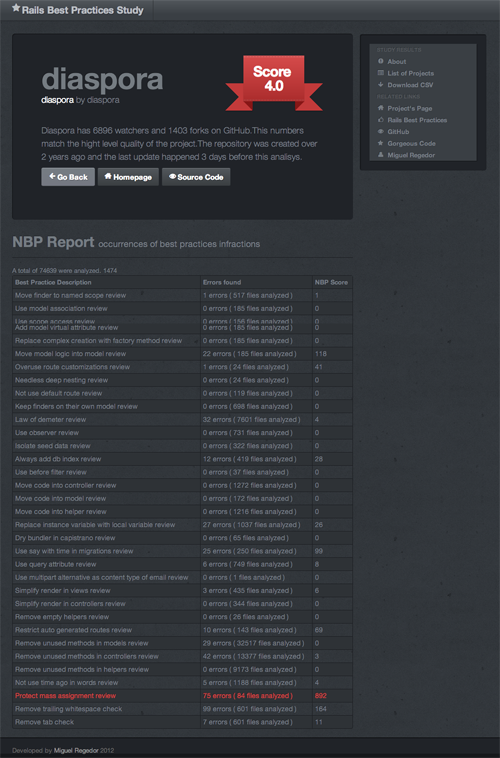
\includegraphics[scale=0.75]{Images/rbp_s}
\end{figure}

The mentioned application was developed using Ruby on Rails, and it is actually possible to consult an extensive list of analyzed projects online at \url{app.study.gourgeouscode.com}. For each project, a page like the table in Figure~\ref{fig:rbp_s} is generated, 
which contains the overall score, a brief possible explanation for the actual score, and a table pointing out the 
NBPs found. If a row is shown in red, it indicates that the score of the project was significantly lowered because 
it does not follow that specific best practice. In other words, this should be the first place to improve the code,
which will also increase the quality of the project.

This application was the ultimate result of these studies.












